\section{Results}

\subsection{Distinctiveness}

%\begin{figure*}[t]
%\centerline{% 
%		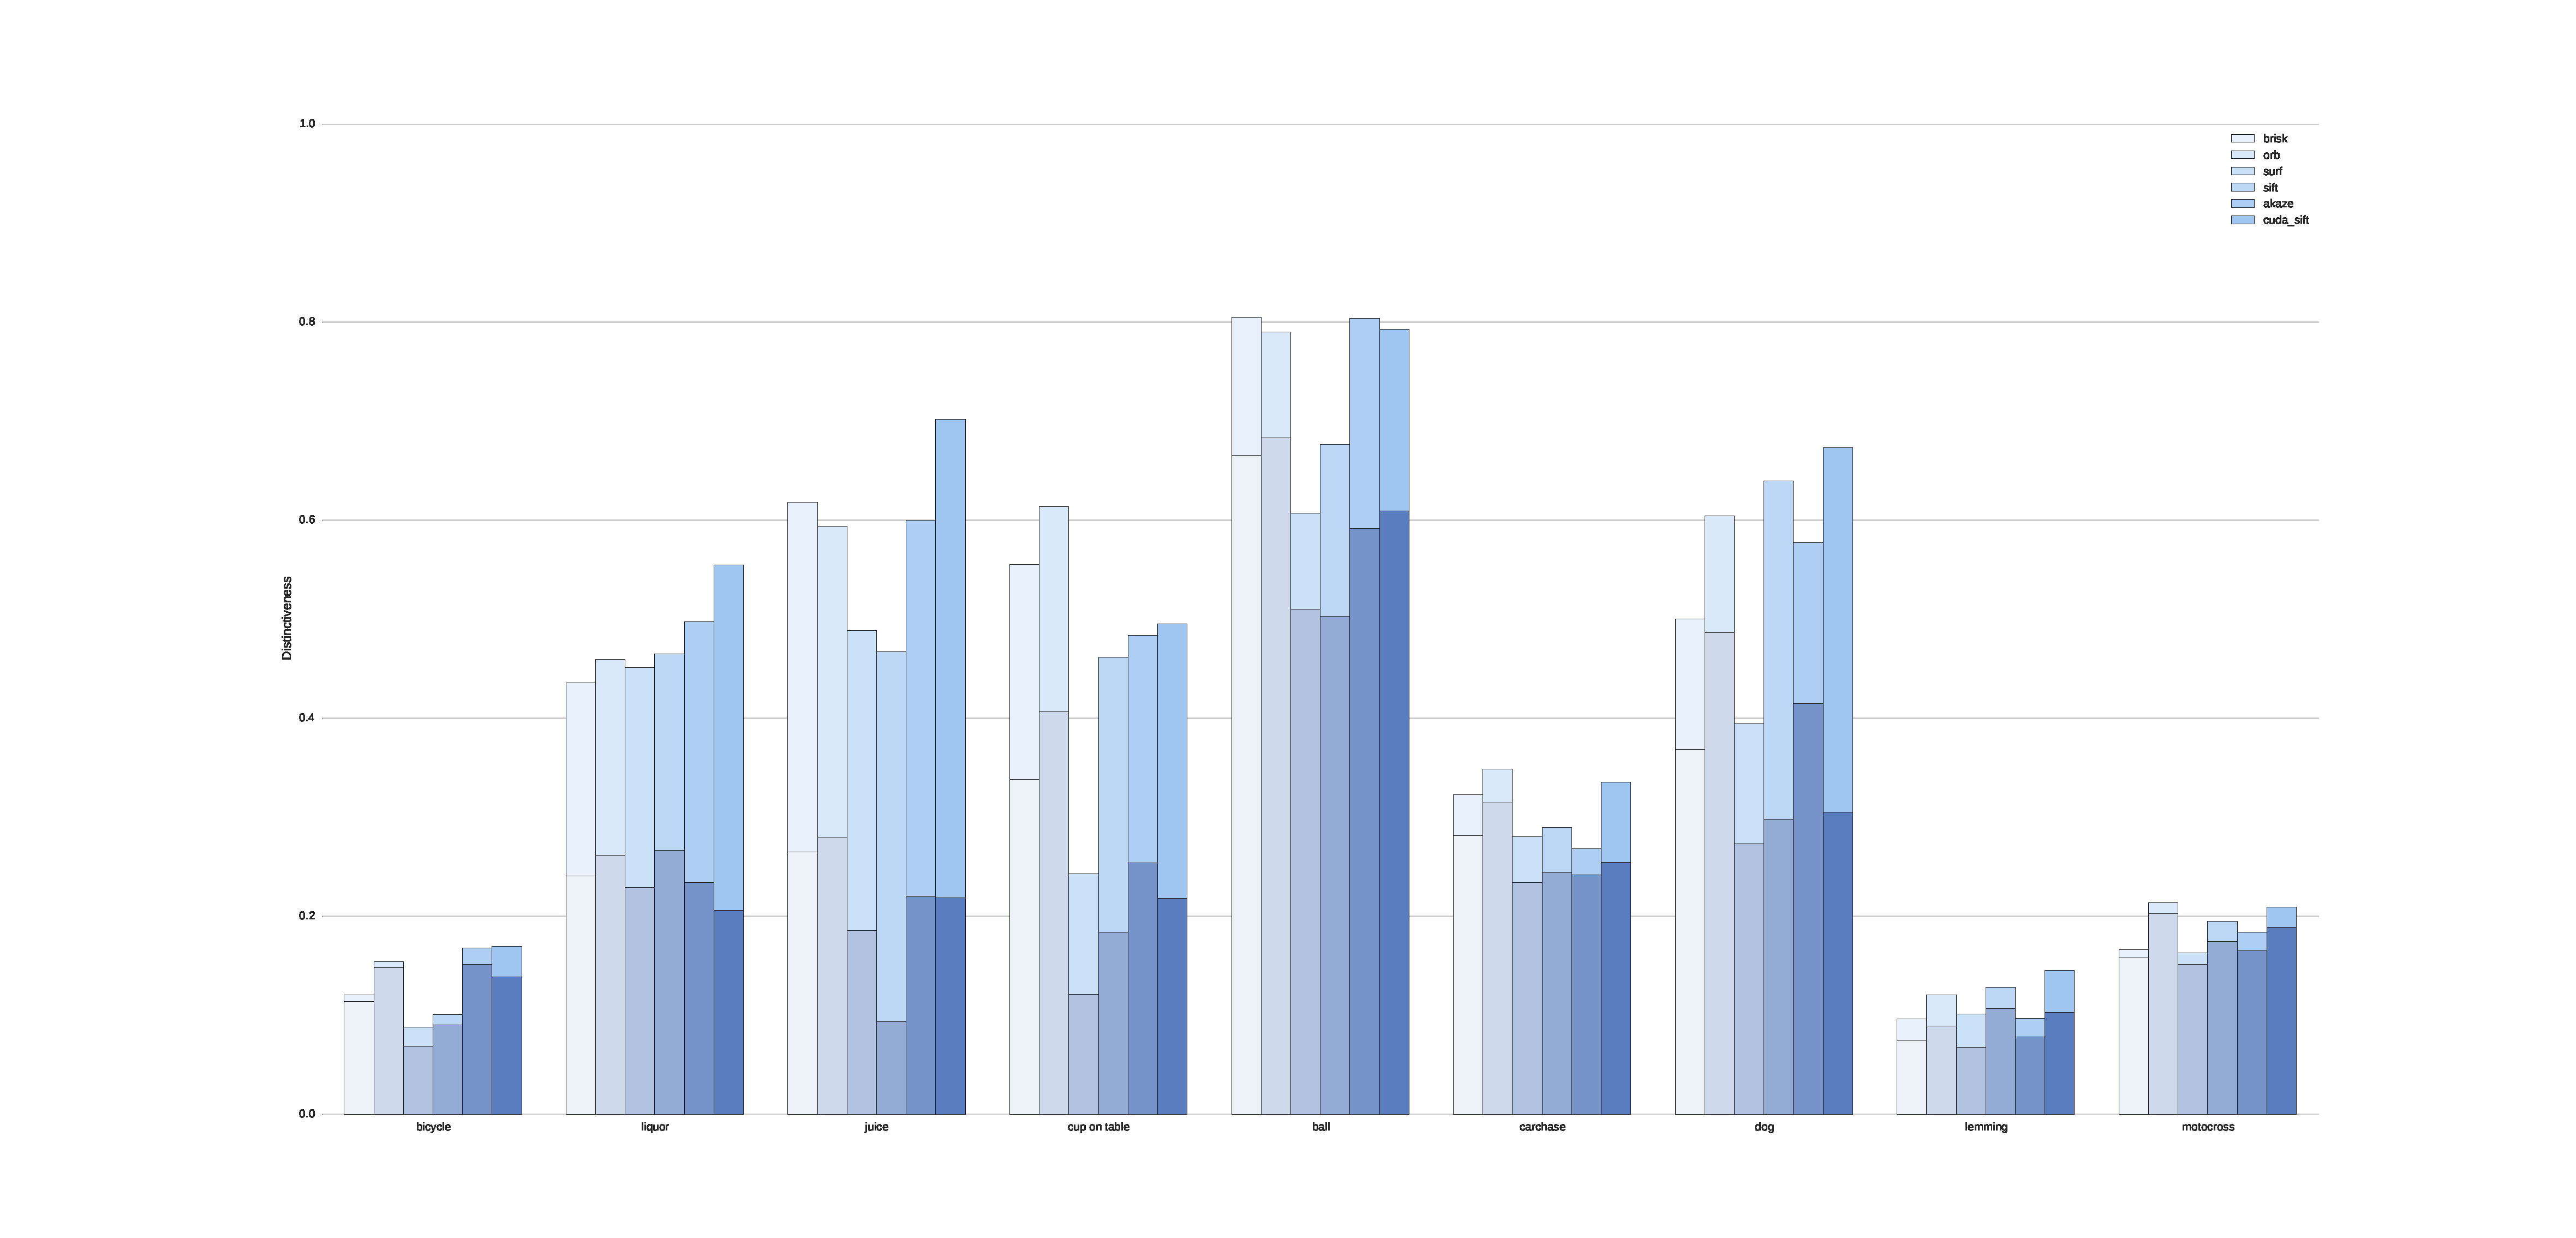
\includegraphics[width=0.98\linewidth]{imgs/distinctivenessTP.pdf}}
%    \vspace{-2mm} 
%	\caption{Examples taken from the dataset showing the ratio of true positives and ambiguous true positives. The lighter color bars show the number of true positives that will actually pass the second best result test.}
%	\label{fig:distinctiveness}
%\end{figure*}

Tab.~\ref{table:tp_ratio} shows the average number of key-points extracted, descriptors belonging to the object to track and the ratio of true positives (TP), false positives (FP) and true positives that pass the second best match ratio check (TTP). It is interesting to notice that BRISK, ORB and SIFT extract a higher number of feature descriptors in general. In particular BRISK and ORB have a higher number of key-points extracted within the area of the object. However, looking at the average amount of true positives it can be seen that the best performing descriptors are AKAZE and the implementation of SIFT on the GPU. This is a first indicator of the quality of the descriptors extracted. Moreover, it can be noticed that the true positives are also more distinctive in the case of AKAZE and SIFT since the number of TTP is higher.

\begin{table}[t]
\caption{Average number of true positives, and total feature extracted.}
\centerline{% 
		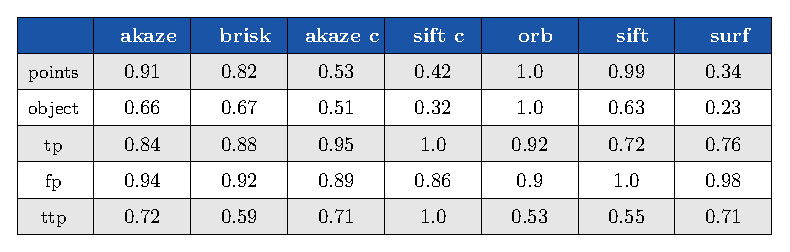
\includegraphics[width=0.98\linewidth]{tables/descriptivness_ratio.pdf}}
    \vspace{-2mm} 
	\label{table:tp_ratio}
\end{table}

\subsection{Tracking accuracy}

As explained in the previous section \ref{sec:accuracy}, we evaluated the performance of the feature descriptors running our tracker and calculating the overlap measure for low, medium and high accuracy requirements. It can be noticed in our results (table~\ref{table:taccuracy}) that AKAZE, BRISK, ORB and SIFT have comparable results. Even if BRISK and ORB has been proven to be less descriptive, the higher amount of weak descriptors extracted seems to compensate this weakness. Upon inspection we noticed that a higher number of features makes the difference when the object to track undergoes drastic changes in scale. In particular we noticed that AKAZE, more than SIFT, suffers the change in scale (e.g. Fig.~\ref{fig:tracking_results_scale}). 

\begin{figure}[t]
	\vspace{2mm}
\centerline{%
	\subfigure{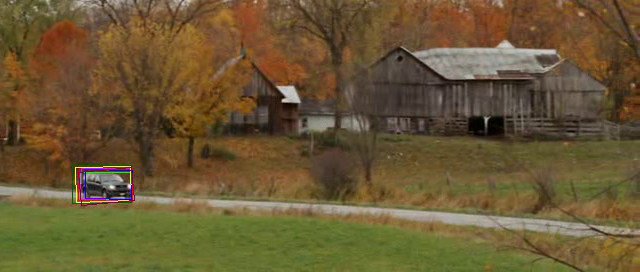
\includegraphics[width=0.48\linewidth]{imgs/results/ex3.png}}
	\subfigure{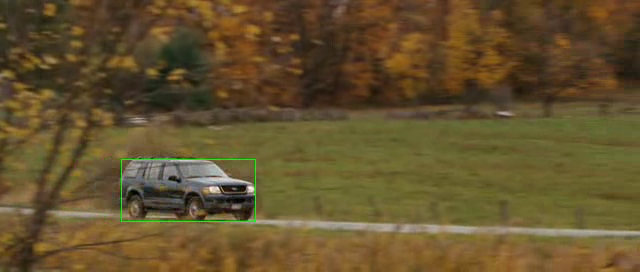
\includegraphics[width=0.48\linewidth]{imgs/results/ex4.png}}}
	\vspace{-2mm}
\caption{Despite most of the descriptors are scale invariant this example shows their weakness in working with drastic scale change.}
\vspace{-3mm}
\label{fig:tracking_results_scale}
\end{figure} 

\subsection{Tracking performance}

We evaluate the performance of each feature descriptor in three different steps: detection, computation and matching. Fig.~\ref{fig:speed} shows the overall results on the dataset. It is interesting to notice that despite AKAZE exploits multiple core on the CPU, its detection part is expensive due to the non-linear filtering. Brisk and ORB are faster but then the matching step is more expensive given the higher number of features extracted. Please note that this numbers are only informative. We think that it is not fair to compare multi-threaded implementations (e.g AKAZE) with single threaded (SIFT) or GPU implementation (SIFT).

\begin{figure}[t]
	\vspace{2mm}
\centerline{%
	\subfigure{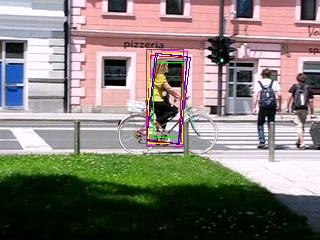
\includegraphics[width=0.48\linewidth]{imgs/results/ex1.png}}
	\subfigure{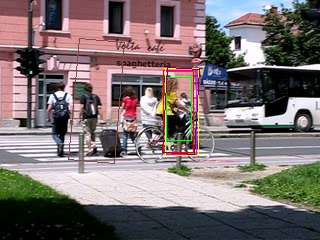
\includegraphics[width=0.48\linewidth]{imgs/results/ex2.png}}}
	\vspace{-2mm}
\centerline{%
	\subfigure{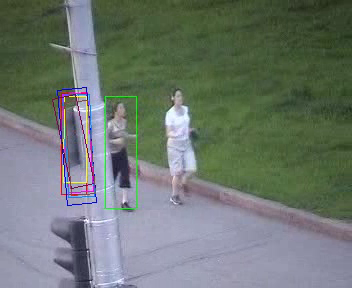
\includegraphics[width=0.48\linewidth]{imgs/results/ex5.png}}
	\subfigure{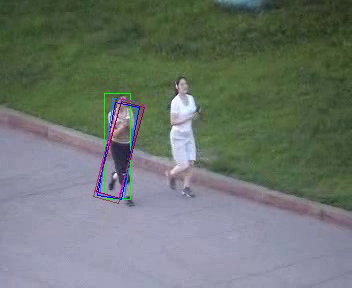
\includegraphics[width=0.48\linewidth]{imgs/results/ex6.png}}}
\caption{Examples showing the behaviour of the feature descriptors upon occlusion. Upon recovery from track loss more descriptive descriptors allow the tracker to recover faster.}
\vspace{-3mm}
\label{fig:tracking_results}
\end{figure}

\begin{figure}[b]
	%\vspace{-2mm}
	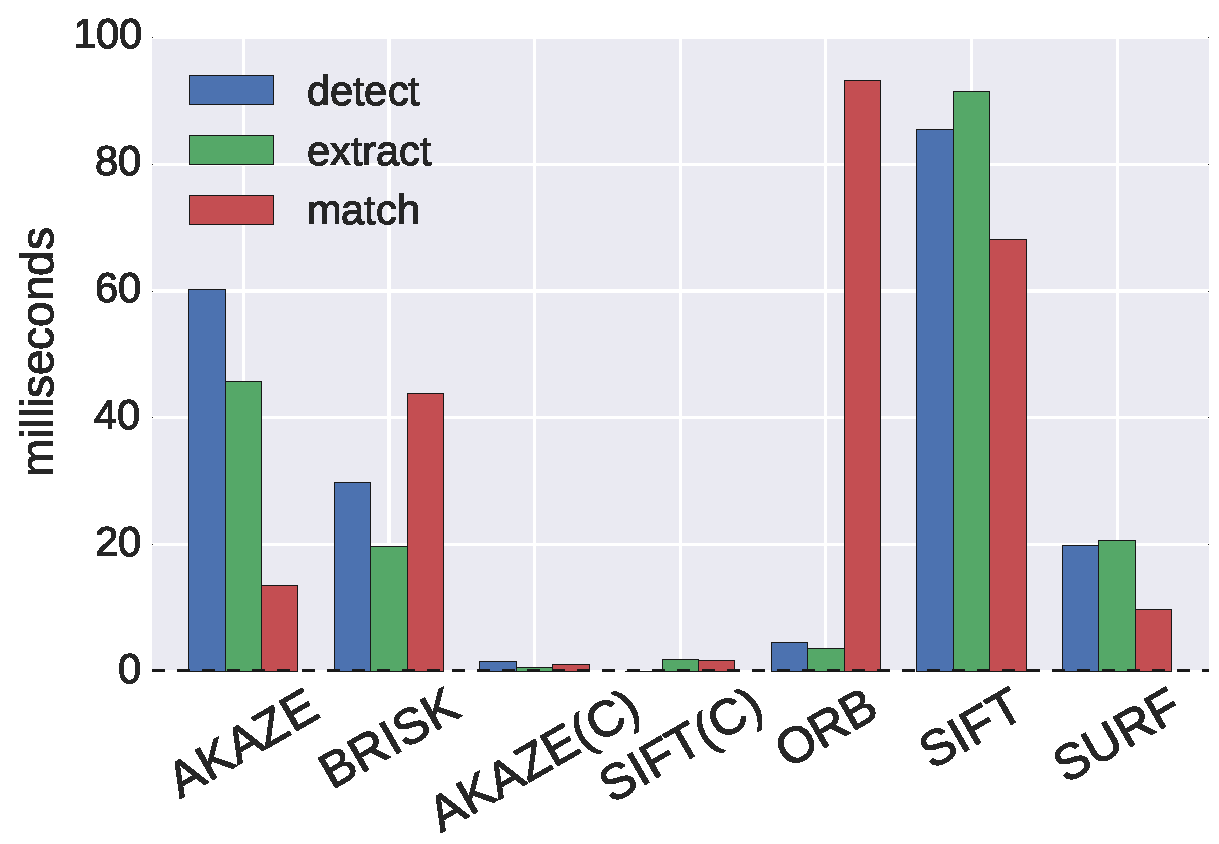
\includegraphics[width=0.95\linewidth]{imgs/performances.pdf}
\vspace{-2.5mm}	
\caption{Performance of the compute,detect and match steps of each feature descriptor.}
\label{fig:speed}
\end{figure}

\begin{table}
\caption{Average time spent on a single frame by the tracker.}
	%\vspace{-2mm}
	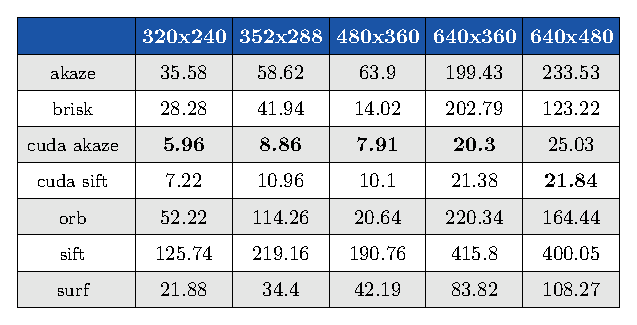
\includegraphics[width=0.95\linewidth]{tables/resolution_times.pdf}
\vspace{-2.5mm}	
\label{fig:fps}
\end{table}


\begin{figure}
	%\vspace{-2mm}
	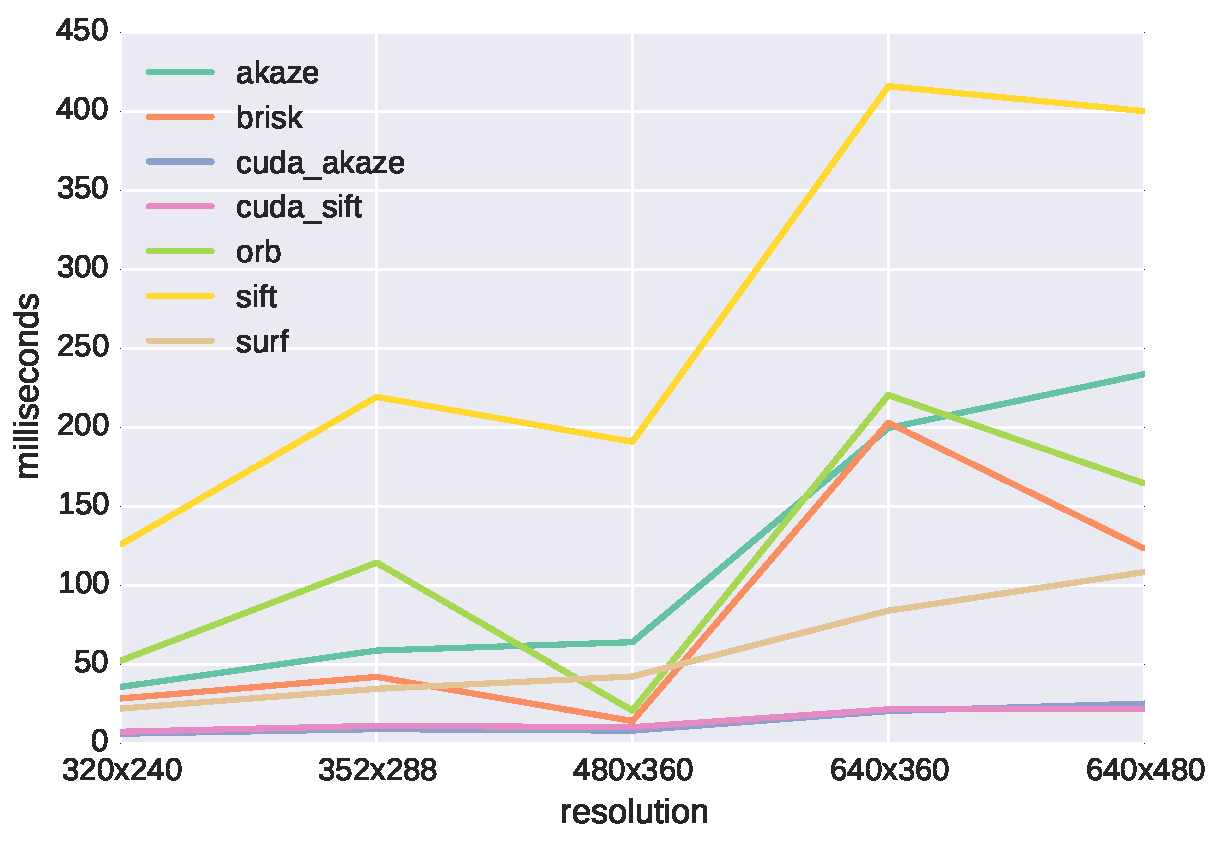
\includegraphics[width=0.95\linewidth]{imgs/tracker_fps.pdf}
\vspace{-2.5mm}	
\caption{Performance of the tracker using each feature descriptor.}
\label{fig:speed}
\end{figure}




\begin{table*}[h]
\caption{Tracking results with low,medium and high accuracy requirements. The high number of key points extracted by ORB or BRISK compensate their weak descriptors. This comes with a cost in performance.} 
\centerline{%
		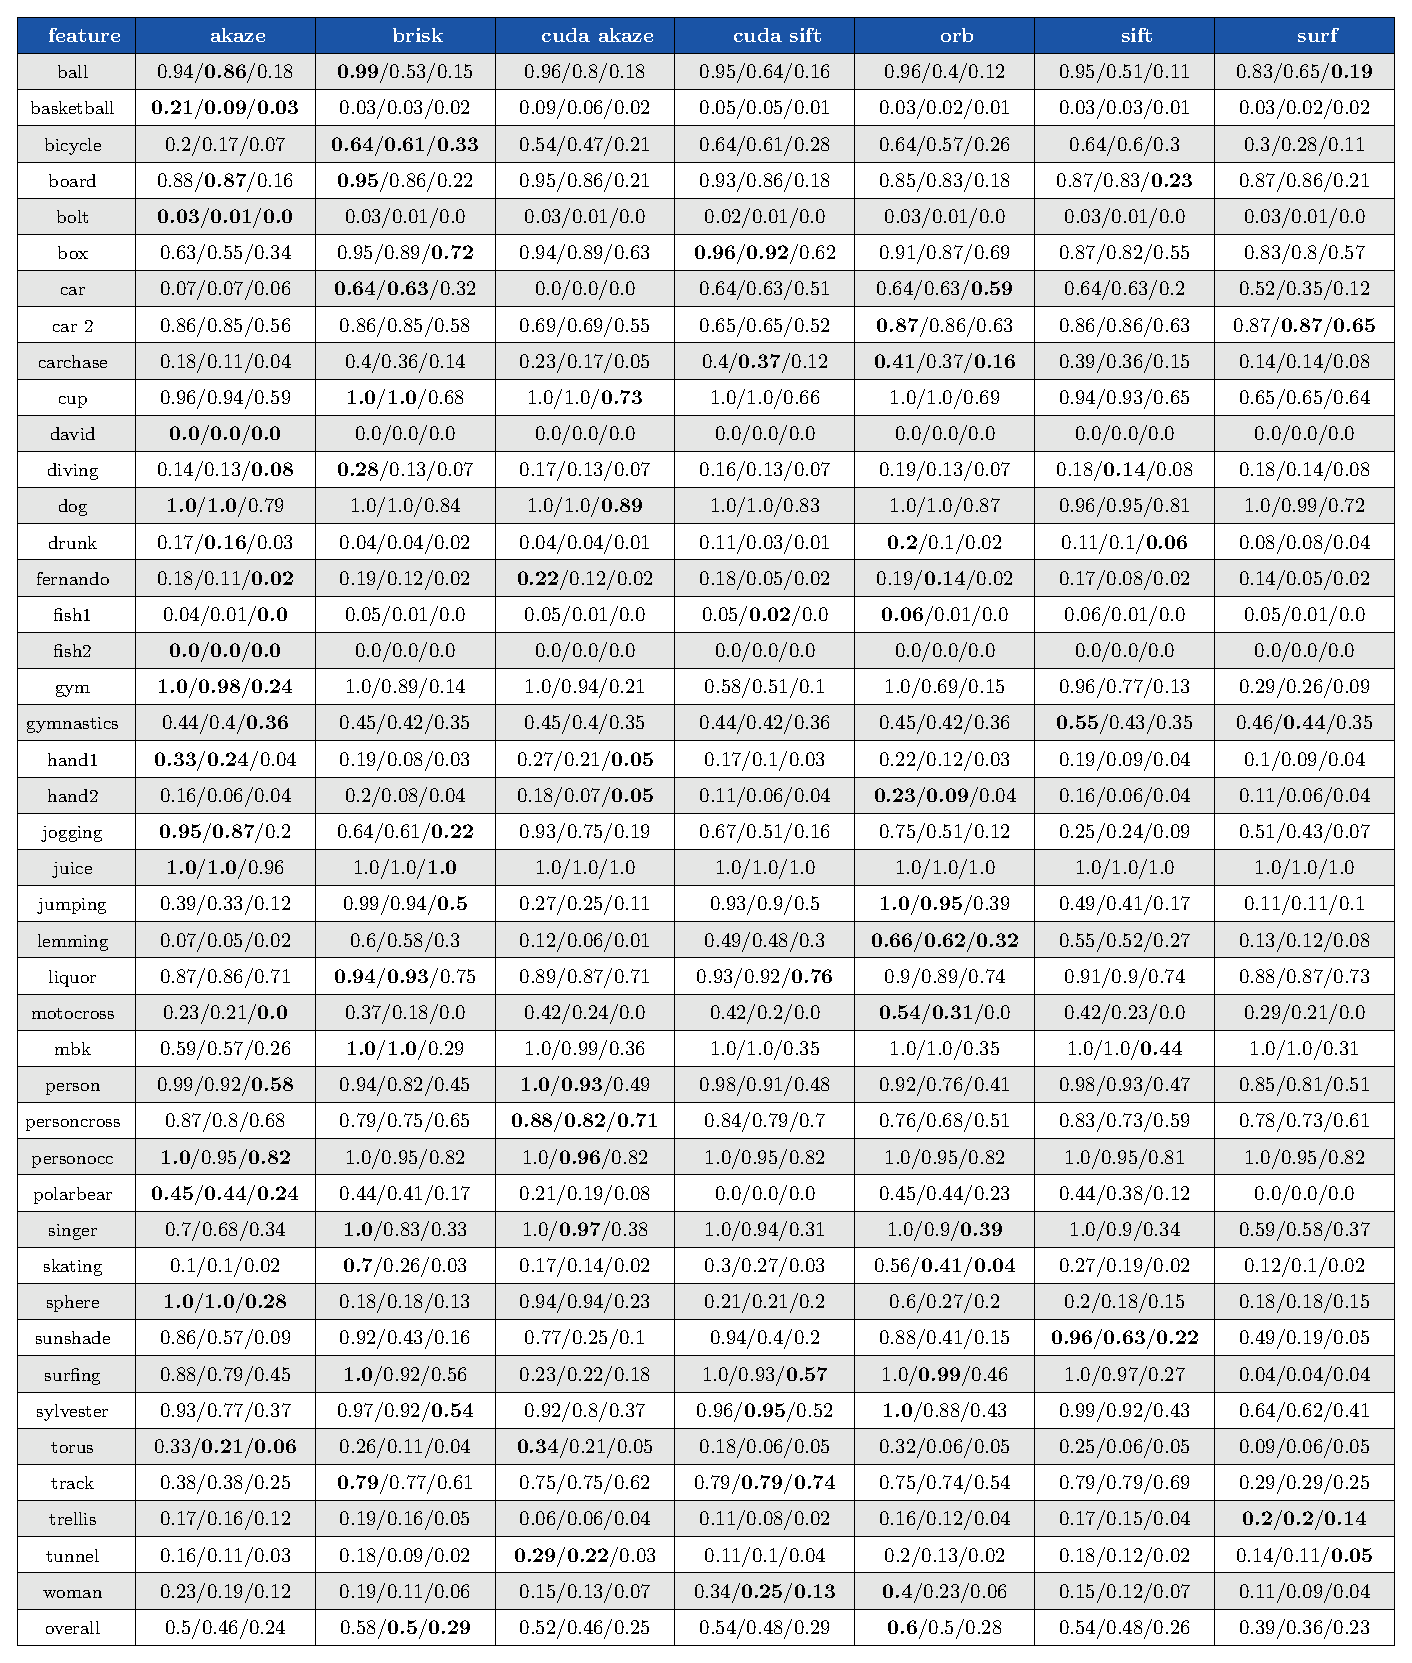
\includegraphics[width=0.98\linewidth]{tables/tracking_precision.pdf}}
    \vspace{-2mm} 
	\label{table:taccuracy}
\end{table*}